\documentclass[a4paper]{book}
\usepackage{a4wide}
\usepackage{makeidx}
\usepackage{graphicx}
\usepackage{multicol}
\usepackage{float}
\usepackage{listings}
\usepackage{color}
\usepackage{textcomp}
\usepackage{alltt}
\usepackage{times}
\usepackage{ifpdf}
\ifpdf
\usepackage[pdftex,
            pagebackref=true,
            colorlinks=true,
            linkcolor=blue,
            unicode
           ]{hyperref}
\else
\usepackage[ps2pdf,
            pagebackref=true,
            colorlinks=true,
            linkcolor=blue,
            unicode
           ]{hyperref}
\usepackage{pspicture}
\fi
\usepackage[utf8]{inputenc}
\usepackage{doxygen}
\lstset{language=C++,inputencoding=utf8,basicstyle=\footnotesize,breaklines=true,breakatwhitespace=true,tabsize=8,numbers=left }
\makeindex
\setcounter{tocdepth}{3}
\renewcommand{\footrulewidth}{0.4pt}
\begin{document}
\hypersetup{pageanchor=false}
\begin{titlepage}
\vspace*{7cm}
\begin{center}
{\Large PhpLib }\\
\vspace*{1cm}
{\large Generated by Doxygen 1.6.3}\\
\vspace*{0.5cm}
{\small Fri Nov 22 16:32:02 2013}\\
\end{center}
\end{titlepage}
\clearemptydoublepage
\pagenumbering{roman}
\tableofcontents
\clearemptydoublepage
\pagenumbering{arabic}
\hypersetup{pageanchor=true}
\chapter{Class Index}
\section{Class Hierarchy}
This inheritance list is sorted roughly, but not completely, alphabetically:\begin{DoxyCompactList}
\item \contentsline{section}{Object}{\pageref{classObject}}{}
\begin{DoxyCompactList}
\item \contentsline{section}{String}{\pageref{classString}}{}
\end{DoxyCompactList}
\end{DoxyCompactList}

\chapter{Class Index}
\section{Class List}
Here are the classes, structs, unions and interfaces with brief descriptions:\begin{DoxyCompactList}
\item\contentsline{section}{\hyperlink{classObject}{Object} }{\pageref{classObject}}{}
\item\contentsline{section}{\hyperlink{classString}{String} }{\pageref{classString}}{}
\end{DoxyCompactList}

\chapter{Class Documentation}
\hypertarget{classObject}{
\section{Object Class Reference}
\label{classObject}\index{Object@{Object}}
}
Inheritance diagram for Object:\begin{figure}[H]
\begin{center}
\leavevmode
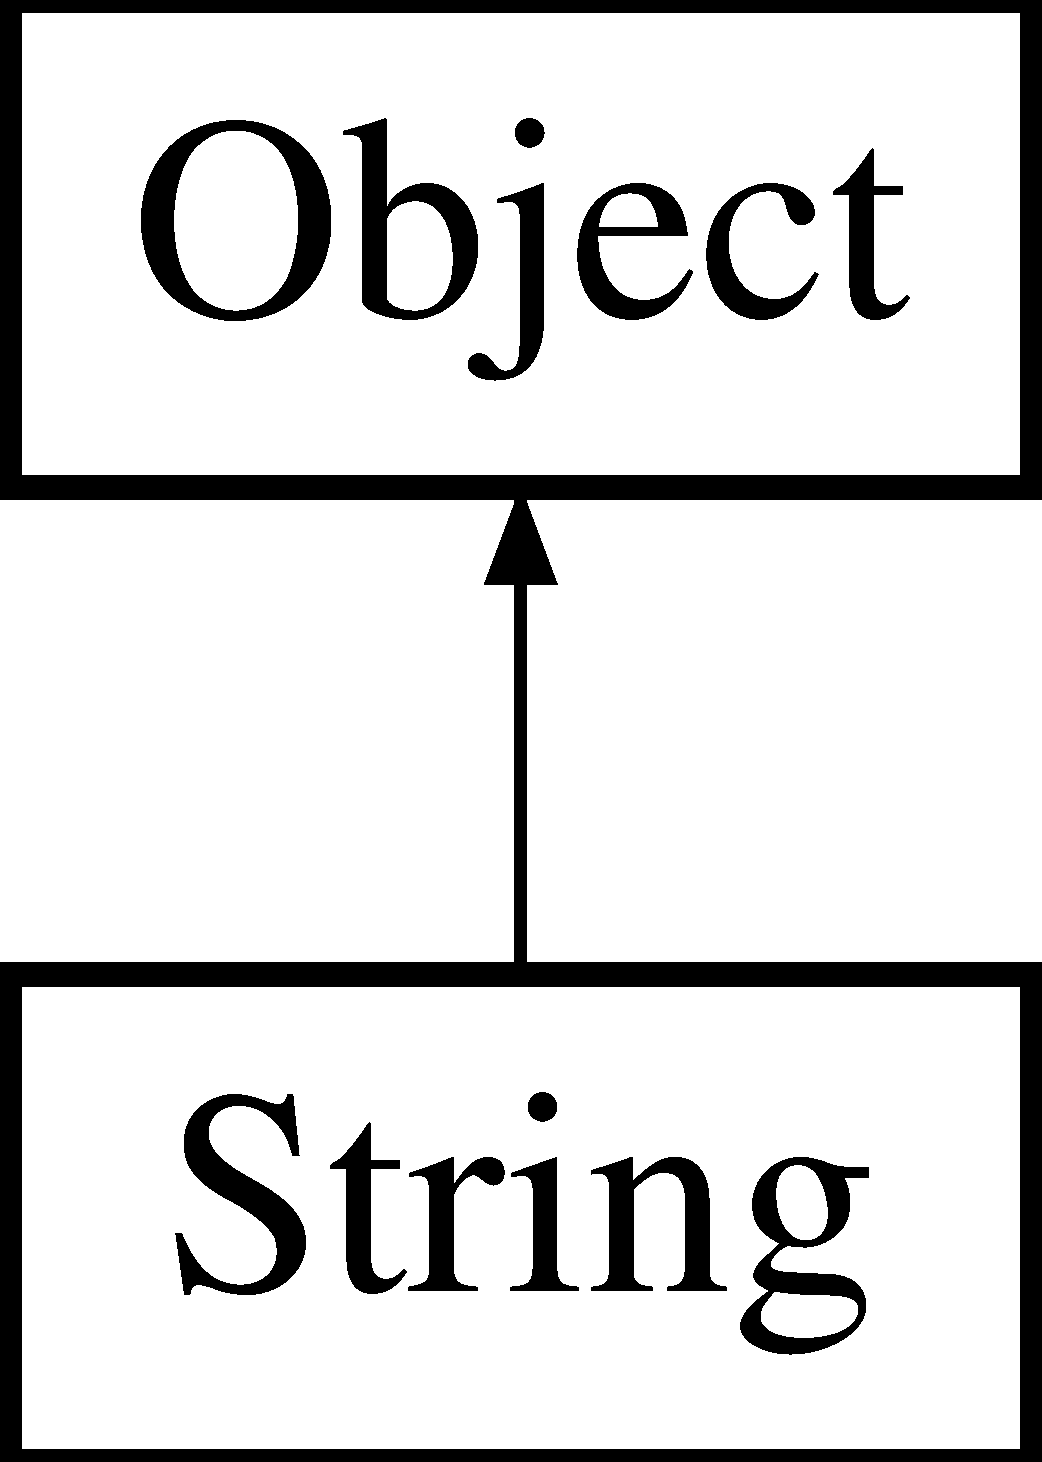
\includegraphics[height=2cm]{classObject}
\end{center}
\end{figure}
\subsection*{Public Member Functions}
\begin{DoxyCompactItemize}
\item 
\hypertarget{classObject_a624c31df2f7cadf888886e0407f26bbe}{
{\bfseries toString} ()}
\label{classObject_a624c31df2f7cadf888886e0407f26bbe}

\end{DoxyCompactItemize}


The documentation for this class was generated from the following file:\begin{DoxyCompactItemize}
\item 
Object.php\end{DoxyCompactItemize}

\hypertarget{classString}{
\section{String Class Reference}
\label{classString}\index{String@{String}}
}
Inheritance diagram for String:\begin{figure}[H]
\begin{center}
\leavevmode
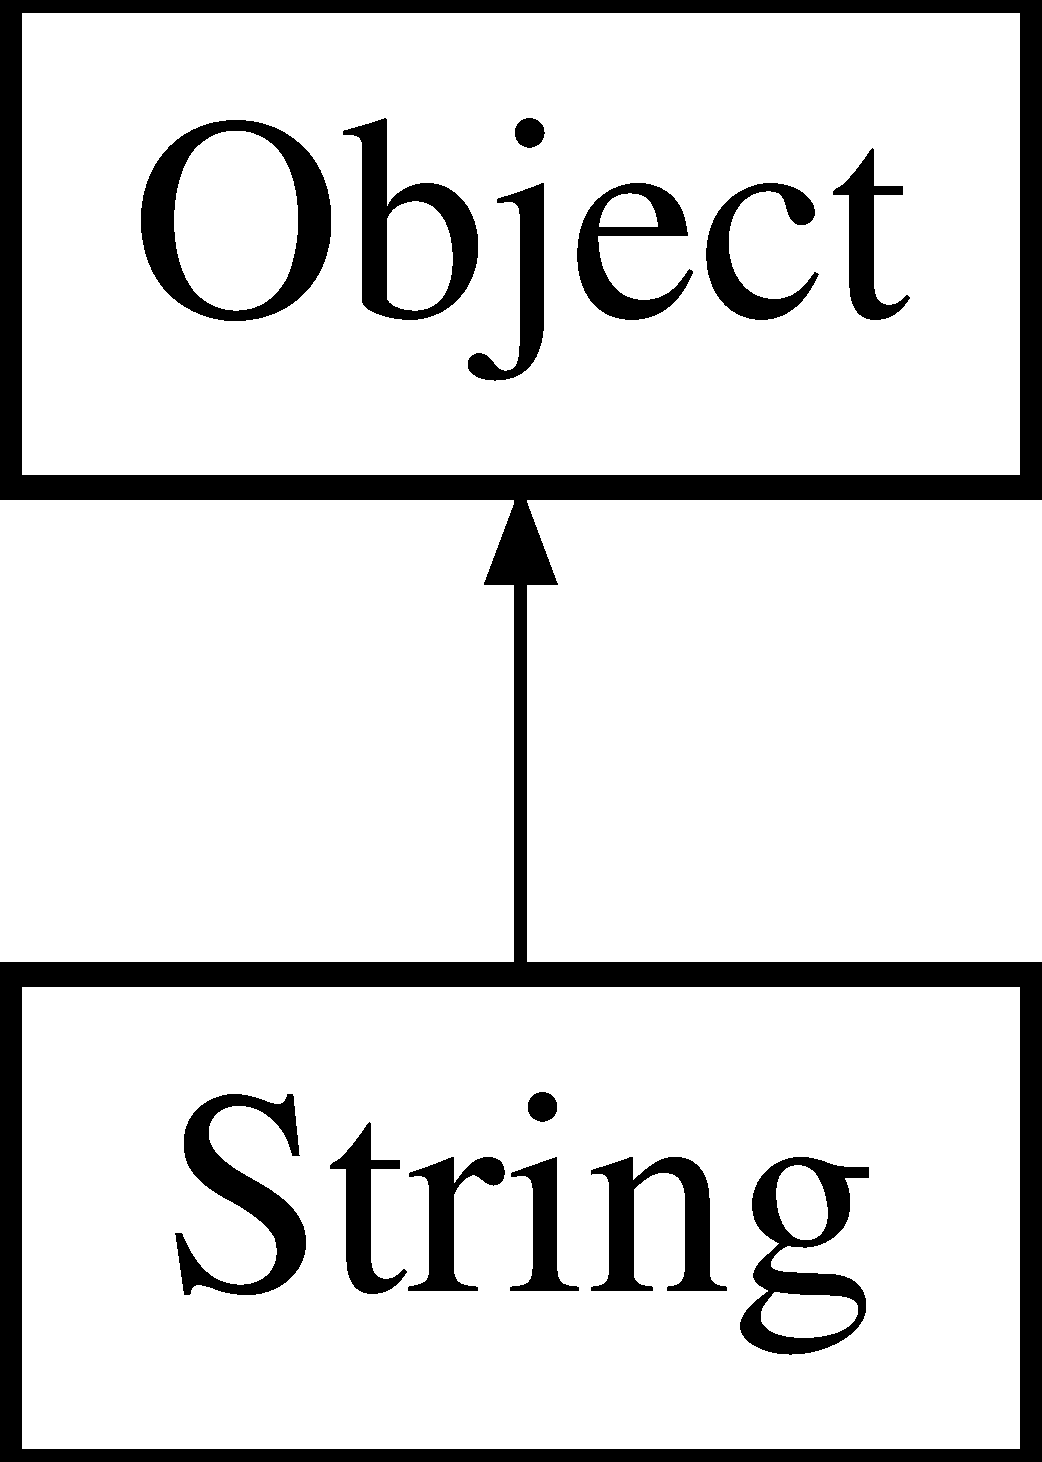
\includegraphics[height=2cm]{classString}
\end{center}
\end{figure}
\subsection*{Public Member Functions}
\begin{DoxyCompactItemize}
\item 
\hypertarget{classString_a0b799cf9b80e4cff537c1f97782f96fd}{
{\bfseries \_\-\_\-construct} (\$str=null)}
\label{classString_a0b799cf9b80e4cff537c1f97782f96fd}

\item 
\hyperlink{classString_a5069041d10f95e4ec9a4be3cd17ab180}{indexOf} (\$str, \$offset=0)
\item 
\hyperlink{classString_a1c8a1df4030974f7ae48f59c1a9dca80}{indexOfAny} (\$chars, \$offset=0)
\item 
\hyperlink{classString_a18806fe790375032e3fb268f649914d7}{lastIndexOf} (\$str, \$offset=0)
\item 
\hyperlink{classString_adbe9cb0e51c46bd16881923a7a3d2e4a}{lastIndexOfAny} (\$chars, \$offset=0)
\item 
\hyperlink{classString_ae7254778c39de64320813d1da9f2f276}{bytes} ()
\item 
\hyperlink{classString_aa8542443a25479d810d0c580680f685d}{pad} (\$len, \$ch= ' ')
\item 
\hyperlink{classString_ae39386e13e0e87cff555bfaea20ce656}{padLeft} (\$len, \$ch= ' ')
\item 
\hyperlink{classString_a8ab0df0a7bbe4d99b84356403abf946f}{padRight} (\$len, \$ch= ' ')
\item 
\hyperlink{classString_ac3a075e35b0f39698230957bc7d0172d}{trim} ()
\item 
\hyperlink{classString_a316e68c5acc7716e4aac01c78a1b5063}{trimEnd} ()
\item 
\hyperlink{classString_a34b1f94648606639f31a7596445ff52e}{trimStart} ()
\item 
\hypertarget{classString_adc4f1d6a5b06b6c610f89131e7b8e403}{
{\bfseries replace} (\$search, \$replace)}
\label{classString_adc4f1d6a5b06b6c610f89131e7b8e403}

\item 
\hypertarget{classString_a0ebde07b97b307aedc7f1f17633b90b1}{
{\bfseries remove} (\$offset, \$len=null)}
\label{classString_a0ebde07b97b307aedc7f1f17633b90b1}

\item 
\hyperlink{classString_a459b87eb0e1fd06e68eb58b18ad11897}{contains} (\$str)
\item 
\hyperlink{classString_aa3256858bec84d6ec1d3b7184725f8bd}{endsWith} (\$str)
\item 
\hyperlink{classString_a0ab7fda4a4bc07fcc3ad0eb94cb96b22}{startsWith} (\$str)
\item 
\hypertarget{classString_a680db6e27d0ad3a50aaf779476402def}{
{\bfseries format} (\$format)}
\label{classString_a680db6e27d0ad3a50aaf779476402def}

\item 
\hyperlink{classString_a70de74664e69b6e2fc93d231173df0d2}{lower} ()
\item 
\hyperlink{classString_a07d720a3ea80bbc85f7424d2d7c27701}{upper} ()
\item 
\hyperlink{classString_afa58fa9927bc0240baf185917c849245}{len} ()
\item 
\hyperlink{classString_a47b2739889b38abb582c4eee7d010f91}{rev} ()
\item 
\hyperlink{classString_a23eb86e0ad225b29dd3e02e637a42c37}{sub} (\$offset, \$length=null)
\item 
\hypertarget{classString_af1ceaa53461e40a69de4f14a115d7d56}{
{\bfseries split} (\$pattern, \$limit=-\/1)}
\label{classString_af1ceaa53461e40a69de4f14a115d7d56}

\item 
\hypertarget{classString_abe7d7e1e2b57ab7dcd01d8e2d1d53148}{
{\bfseries insert} (\$offset, \$str)}
\label{classString_abe7d7e1e2b57ab7dcd01d8e2d1d53148}

\item 
\hypertarget{classString_abacf7b1614b42312f4f49ca064980139}{
{\bfseries toArray} (\$offset=0, \$len=null)}
\label{classString_abacf7b1614b42312f4f49ca064980139}

\item 
\hypertarget{classString_aa7ef98a0c1a4b8b375baf8791e7b773c}{
{\bfseries toString} ()}
\label{classString_aa7ef98a0c1a4b8b375baf8791e7b773c}

\item 
\hypertarget{classString_a6a17056cddb17560a093b846c6168537}{
{\bfseries offsetSet} (\$offset, \$value)}
\label{classString_a6a17056cddb17560a093b846c6168537}

\item 
\hypertarget{classString_a4627964e8bc80f485b4b7c1b1c609820}{
{\bfseries offsetGet} (\$offset)}
\label{classString_a4627964e8bc80f485b4b7c1b1c609820}

\item 
\hypertarget{classString_a0ad487f2acca3753cd9d42cf9325225e}{
{\bfseries offsetExists} (\$offset)}
\label{classString_a0ad487f2acca3753cd9d42cf9325225e}

\item 
\hypertarget{classString_af12691beca61c36ac057a8515b2f4bfe}{
{\bfseries offsetUnset} (\$offset)}
\label{classString_af12691beca61c36ac057a8515b2f4bfe}

\end{DoxyCompactItemize}


\subsection{Member Function Documentation}
\hypertarget{classString_ae7254778c39de64320813d1da9f2f276}{
\index{String@{String}!bytes@{bytes}}
\index{bytes@{bytes}!String@{String}}
\subsubsection[{bytes}]{\setlength{\rightskip}{0pt plus 5cm}String::bytes ()}}
\label{classString_ae7254778c39de64320813d1da9f2f276}
Gets the number of bytes the string takes \begin{DoxyReturn}{Returns}
The number of bytes the string takes 
\end{DoxyReturn}
\hypertarget{classString_a459b87eb0e1fd06e68eb58b18ad11897}{
\index{String@{String}!contains@{contains}}
\index{contains@{contains}!String@{String}}
\subsubsection[{contains}]{\setlength{\rightskip}{0pt plus 5cm}String::contains (\$ {\em str})}}
\label{classString_a459b87eb0e1fd06e68eb58b18ad11897}
Checks whether the \hyperlink{classString}{String} contains the given string 
\begin{DoxyParams}{Parameters}
\item[{\em str}]The string to look for \end{DoxyParams}
\begin{DoxyReturn}{Returns}
A boolean to indicate whether the string exists 
\end{DoxyReturn}
\hypertarget{classString_aa3256858bec84d6ec1d3b7184725f8bd}{
\index{String@{String}!endsWith@{endsWith}}
\index{endsWith@{endsWith}!String@{String}}
\subsubsection[{endsWith}]{\setlength{\rightskip}{0pt plus 5cm}String::endsWith (\$ {\em str})}}
\label{classString_aa3256858bec84d6ec1d3b7184725f8bd}
Checks wether the \hyperlink{classString}{String} ends with the given string 
\begin{DoxyParams}{Parameters}
\item[{\em str}]The string it should end with \end{DoxyParams}
\begin{DoxyReturn}{Returns}
A boolean to indicate wether the string ends with the given one 
\end{DoxyReturn}
\hypertarget{classString_a5069041d10f95e4ec9a4be3cd17ab180}{
\index{String@{String}!indexOf@{indexOf}}
\index{indexOf@{indexOf}!String@{String}}
\subsubsection[{indexOf}]{\setlength{\rightskip}{0pt plus 5cm}String::indexOf (\$ {\em str}, \/  \$ {\em offset} = {\ttfamily 0})}}
\label{classString_a5069041d10f95e4ec9a4be3cd17ab180}
Searches for the first occurrence of the string and returnd the position 
\begin{DoxyParams}{Parameters}
\item[{\em str}]The string to find \item[{\em offset}]A zero-\/based offset to start the search from \end{DoxyParams}
\begin{DoxyReturn}{Returns}
The zero-\/based position where the string was found or false if not found 
\end{DoxyReturn}
\hypertarget{classString_a1c8a1df4030974f7ae48f59c1a9dca80}{
\index{String@{String}!indexOfAny@{indexOfAny}}
\index{indexOfAny@{indexOfAny}!String@{String}}
\subsubsection[{indexOfAny}]{\setlength{\rightskip}{0pt plus 5cm}String::indexOfAny (\$ {\em chars}, \/  \$ {\em offset} = {\ttfamily 0})}}
\label{classString_a1c8a1df4030974f7ae48f59c1a9dca80}
Searches for the first occurrence of any given character and returns the position 
\begin{DoxyParams}{Parameters}
\item[{\em chars}]The array of characters to find \item[{\em offset}]A zero-\/based offset to start the search from \end{DoxyParams}
\begin{DoxyReturn}{Returns}
The zero-\/based position where a character was found or false if not found 
\end{DoxyReturn}
\hypertarget{classString_a18806fe790375032e3fb268f649914d7}{
\index{String@{String}!lastIndexOf@{lastIndexOf}}
\index{lastIndexOf@{lastIndexOf}!String@{String}}
\subsubsection[{lastIndexOf}]{\setlength{\rightskip}{0pt plus 5cm}String::lastIndexOf (\$ {\em str}, \/  \$ {\em offset} = {\ttfamily 0})}}
\label{classString_a18806fe790375032e3fb268f649914d7}
Searches for the last occurrence of the string and returns the position 
\begin{DoxyParams}{Parameters}
\item[{\em str}]The string to find \item[{\em offset}]A zero-\/based offset to start the search from TODO \end{DoxyParams}
\begin{DoxyReturn}{Returns}
The zero-\/based position where the string was found or false if not found 
\end{DoxyReturn}
\hypertarget{classString_adbe9cb0e51c46bd16881923a7a3d2e4a}{
\index{String@{String}!lastIndexOfAny@{lastIndexOfAny}}
\index{lastIndexOfAny@{lastIndexOfAny}!String@{String}}
\subsubsection[{lastIndexOfAny}]{\setlength{\rightskip}{0pt plus 5cm}String::lastIndexOfAny (\$ {\em chars}, \/  \$ {\em offset} = {\ttfamily 0})}}
\label{classString_adbe9cb0e51c46bd16881923a7a3d2e4a}
Searches for the last occurrence of any given character and return the position 
\begin{DoxyParams}{Parameters}
\item[{\em chars}]\item[{\em offset}]A zero-\/based offset to start the search from \end{DoxyParams}
\begin{DoxyReturn}{Returns}
The zero-\/based position where a character was found or false if not found 
\end{DoxyReturn}
\hypertarget{classString_afa58fa9927bc0240baf185917c849245}{
\index{String@{String}!len@{len}}
\index{len@{len}!String@{String}}
\subsubsection[{len}]{\setlength{\rightskip}{0pt plus 5cm}String::len ()}}
\label{classString_afa58fa9927bc0240baf185917c849245}
Determines the number of characters contained in the \hyperlink{classString}{String} \begin{DoxyReturn}{Returns}
The number of characters 
\end{DoxyReturn}
\hypertarget{classString_a70de74664e69b6e2fc93d231173df0d2}{
\index{String@{String}!lower@{lower}}
\index{lower@{lower}!String@{String}}
\subsubsection[{lower}]{\setlength{\rightskip}{0pt plus 5cm}String::lower ()}}
\label{classString_a70de74664e69b6e2fc93d231173df0d2}
Creates a new \hyperlink{classString}{String} version with lowercase characters \begin{DoxyReturn}{Returns}
The new lowercase \hyperlink{classString}{String} 
\end{DoxyReturn}
\hypertarget{classString_aa8542443a25479d810d0c580680f685d}{
\index{String@{String}!pad@{pad}}
\index{pad@{pad}!String@{String}}
\subsubsection[{pad}]{\setlength{\rightskip}{0pt plus 5cm}String::pad (\$ {\em len}, \/  \$ {\em ch} = {\ttfamily '~'})}}
\label{classString_aa8542443a25479d810d0c580680f685d}
Creates a new \hyperlink{classString}{String} with equal padding to the left and right, if the padding is odd the right padding is bigger 
\begin{DoxyParams}{Parameters}
\item[{\em len}]The total target length, string and padding \item[{\em ch}]The padding character or string \end{DoxyParams}
\begin{DoxyReturn}{Returns}
A new \hyperlink{classString}{String} containing the old string and the padding 
\end{DoxyReturn}
\hypertarget{classString_ae39386e13e0e87cff555bfaea20ce656}{
\index{String@{String}!padLeft@{padLeft}}
\index{padLeft@{padLeft}!String@{String}}
\subsubsection[{padLeft}]{\setlength{\rightskip}{0pt plus 5cm}String::padLeft (\$ {\em len}, \/  \$ {\em ch} = {\ttfamily '~'})}}
\label{classString_ae39386e13e0e87cff555bfaea20ce656}
Creates a new \hyperlink{classString}{String} with padding to the left 
\begin{DoxyParams}{Parameters}
\item[{\em len}]The total target length, string and padding \item[{\em ch}]The padding character or string \end{DoxyParams}
\begin{DoxyReturn}{Returns}
A new \hyperlink{classString}{String} containing the old string and the padding 
\end{DoxyReturn}
\hypertarget{classString_a8ab0df0a7bbe4d99b84356403abf946f}{
\index{String@{String}!padRight@{padRight}}
\index{padRight@{padRight}!String@{String}}
\subsubsection[{padRight}]{\setlength{\rightskip}{0pt plus 5cm}String::padRight (\$ {\em len}, \/  \$ {\em ch} = {\ttfamily '~'})}}
\label{classString_a8ab0df0a7bbe4d99b84356403abf946f}
Creates a new \hyperlink{classString}{String} with padding to the right 
\begin{DoxyParams}{Parameters}
\item[{\em len}]The total target length, string and padding \item[{\em ch}]The padding character or string \end{DoxyParams}
\begin{DoxyReturn}{Returns}
A new \hyperlink{classString}{String} containing the old string and the padding 
\end{DoxyReturn}
\hypertarget{classString_a47b2739889b38abb582c4eee7d010f91}{
\index{String@{String}!rev@{rev}}
\index{rev@{rev}!String@{String}}
\subsubsection[{rev}]{\setlength{\rightskip}{0pt plus 5cm}String::rev ()}}
\label{classString_a47b2739889b38abb582c4eee7d010f91}
Creates a new reversed version of the \hyperlink{classString}{String} \begin{DoxyReturn}{Returns}
The new reversed \hyperlink{classString}{String} 
\end{DoxyReturn}
\hypertarget{classString_a0ab7fda4a4bc07fcc3ad0eb94cb96b22}{
\index{String@{String}!startsWith@{startsWith}}
\index{startsWith@{startsWith}!String@{String}}
\subsubsection[{startsWith}]{\setlength{\rightskip}{0pt plus 5cm}String::startsWith (\$ {\em str})}}
\label{classString_a0ab7fda4a4bc07fcc3ad0eb94cb96b22}
Checks wether the \hyperlink{classString}{String} starts with the given string 
\begin{DoxyParams}{Parameters}
\item[{\em str}]The string it should start with \end{DoxyParams}
\begin{DoxyReturn}{Returns}
A boolean to indicate wether the string starts with the given one 
\end{DoxyReturn}
\hypertarget{classString_a23eb86e0ad225b29dd3e02e637a42c37}{
\index{String@{String}!sub@{sub}}
\index{sub@{sub}!String@{String}}
\subsubsection[{sub}]{\setlength{\rightskip}{0pt plus 5cm}String::sub (\$ {\em offset}, \/  \$ {\em length} = {\ttfamily null})}}
\label{classString_a23eb86e0ad225b29dd3e02e637a42c37}
Creates a copy of a portion of the \hyperlink{classString}{String} 
\begin{DoxyParams}{Parameters}
\item[{\em offset}]The zero-\/based start position \item[{\em lengh}]The length of the portion \end{DoxyParams}
\begin{DoxyReturn}{Returns}
A new \hyperlink{classString}{String} containing only the portion of the \hyperlink{classString}{String} 
\end{DoxyReturn}
\hypertarget{classString_ac3a075e35b0f39698230957bc7d0172d}{
\index{String@{String}!trim@{trim}}
\index{trim@{trim}!String@{String}}
\subsubsection[{trim}]{\setlength{\rightskip}{0pt plus 5cm}String::trim ()}}
\label{classString_ac3a075e35b0f39698230957bc7d0172d}
Creates a new trimmed \hyperlink{classString}{String} without leading or following whitespaces \begin{DoxyReturn}{Returns}
A new trimmed \hyperlink{classString}{String} 
\end{DoxyReturn}
\hypertarget{classString_a316e68c5acc7716e4aac01c78a1b5063}{
\index{String@{String}!trimEnd@{trimEnd}}
\index{trimEnd@{trimEnd}!String@{String}}
\subsubsection[{trimEnd}]{\setlength{\rightskip}{0pt plus 5cm}String::trimEnd ()}}
\label{classString_a316e68c5acc7716e4aac01c78a1b5063}
Creates a new trimmed \hyperlink{classString}{String} without following whitespaces \begin{DoxyReturn}{Returns}
A new trimmed \hyperlink{classString}{String} 
\end{DoxyReturn}
\hypertarget{classString_a34b1f94648606639f31a7596445ff52e}{
\index{String@{String}!trimStart@{trimStart}}
\index{trimStart@{trimStart}!String@{String}}
\subsubsection[{trimStart}]{\setlength{\rightskip}{0pt plus 5cm}String::trimStart ()}}
\label{classString_a34b1f94648606639f31a7596445ff52e}
Creates a new trimmed \hyperlink{classString}{String} without leading whitespaces \begin{DoxyReturn}{Returns}
A new trimmed \hyperlink{classString}{String} 
\end{DoxyReturn}
\hypertarget{classString_a07d720a3ea80bbc85f7424d2d7c27701}{
\index{String@{String}!upper@{upper}}
\index{upper@{upper}!String@{String}}
\subsubsection[{upper}]{\setlength{\rightskip}{0pt plus 5cm}String::upper ()}}
\label{classString_a07d720a3ea80bbc85f7424d2d7c27701}
Creates a new \hyperlink{classString}{String} version with uppercase characters \begin{DoxyReturn}{Returns}
The new uppercase \hyperlink{classString}{String} 
\end{DoxyReturn}


The documentation for this class was generated from the following file:\begin{DoxyCompactItemize}
\item 
String.php\end{DoxyCompactItemize}

\printindex
\end{document}
